\documentclass{article}
\usepackage[utf8]{inputenc}
\usepackage{amsmath}
\usepackage{tcolorbox}
\usepackage{indentfirst}
\usepackage{graphicx}
\usepackage{minted}
\usepackage{float}
\usepackage [english]{babel}
\usepackage [autostyle, english = american]{csquotes}
\MakeOuterQuote{"}

\title{System on a Chip Class Report 3}
\author{Jordan D Edwards}
\date{October 2023}


\begin{document}
	
	\title{Class Report 1
		\\ \large{ELC 4396 System on a Chip}  }
	
	\author{Jordan Edwards \\ Baylor University} %the \\ symbols starts a new line
	\date{October 12, 2023}
	\maketitle
	
	\subsection*{Introduction}
		For this assignment, I completed the setup and basic testing of a vanilla microblaze processor on the Digilent Nexys 4 DDR board. The Vivado hierarchy is shown in Fig. \ref{fig:Vivado}.
		
		\begin{figure}[H]
			\centering
			\includegraphics[width=0.7\linewidth]{"VivadoSC"}
			\caption{Vivado hierarchy}
			\label{fig:Vivado}
		\end{figure}
		
	
	\subsection*{Implementation}
		After importing all necessary driver files in Vivado, I exported the bit file along with the other necessary hardware files into Vitis. Once in Vitis, I set up the project by importing all necessary software files. The resulting project can be see in Fig. \ref{fig:Vitis}.
		
	 \begin{figure}[H]
		\centering
		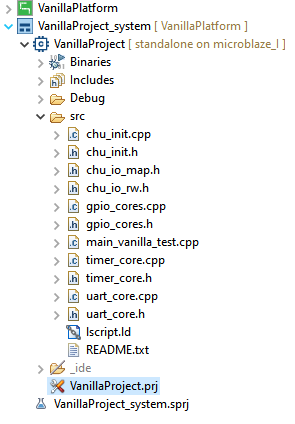
\includegraphics[width=.6\linewidth]{VitisSC}
		\caption{Vitis hierarchy}
		\label{fig:Vitis}
	\end{figure}
	
		With this set up, I altered the default test file so that it would skip the UART test and blink the LEDs at an asymmetric rate. These changes can be seen in Fig. \ref{fig:Code1} and Fig. \ref{fig:Code2} This would allow me to visually confirm that my changes worked correctly. The system is set up such that there is a single bridge module which maps a subset of all available memory to a bank of memory mapped IO modules. These 64 slots each have 32 32 bit registers available to be addressed directly by the processor. At this point, only the LED, switch, UART, and timer modules are implemented. The software in Vitis has special functions to calcuate the absolute memory address for any particular sub-address of any particular module. This allows for each module to be wrapped in a single class which can expose useful methods to the main program, such as sleep\_ms() for the timer.
		
		 \begin{figure}[H]
			\centering
			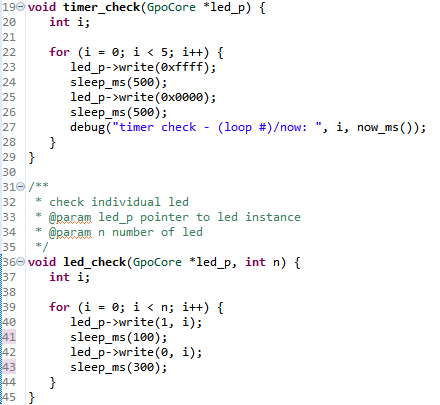
\includegraphics[width=.6\linewidth]{CodeSC1}
			\caption{various test functions}
			\label{fig:Code1}
		\end{figure}
		
		 \begin{figure}[H]
			\centering
			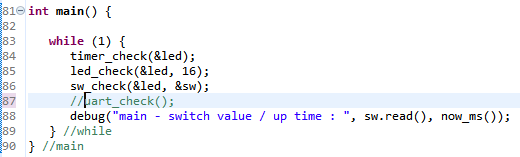
\includegraphics[width=.6\linewidth]{CodeSC2}
			\caption{Main function}
			\label{fig:Code2}
		\end{figure}
	
	\subsection*{Results}
		The code compiled and uploaded successfully to the board. All LEDs blinked at the correct times and for the correct duration. The project works entirely.
\end{document}
